\chapter{Validaci\'on del sistema propuesto}\label{chapter:validation}


\section{Análisis del Espacio de Contraseñas con Discretización Óptima}
\label{subsec:espacio-contrasenas}

El espacio de contraseñas resultante para el sistema \textit{Passpoints} utilizando discretización óptima se calcula mediante la ecuación propuesta en \cite{birget2006graphical}:

\begin{equation}
	P = \left( \frac{a}{6r} \cdot \frac{b}{6r} \right)^c
	\label{eq:espacio-contrasenas}
\end{equation}

donde los parámetros se definen como:

\begin{table}[ht]
	\centering
	\caption{Parámetros del espacio de contraseñas}
	\label{tab:parametros-espacio}
	\begin{tabularx}{0.9\textwidth}{lXl}
		\toprule
		\textbf{Símbolo} & \textbf{Descripción} & \textbf{Dominio} \\
		\midrule
		$a \times b$ & Dimensiones de la imagen (en píxeles) & $\mathbb{Z}^+ \times \mathbb{Z}^+$ \\
		$c$ & Cantidad de puntos seleccionados & $c \geq 5$ \\
		$r$ & Radio de la región de tolerancia & $r \in [8, 32]$ \\
		\bottomrule
	\end{tabularx}
\end{table}

\vspace{0.5cm}

Esta formulación establece que el espacio de contraseñas efectivo $P$ crece exponencialmente con respecto a:
\begin{itemize}
	\item La relación $\frac{a \cdot b}{(6r)^2}$: Densidad de puntos discretizados por área
	\item El número de puntos $c$: Complejidad combinatoria de la secuencia
\end{itemize}

Para una imagen típica de $1024 \times 768$ píxeles con parámetros $r = 16$ y $c = 5$:

\begin{align*}
	P &= \left( \frac{1024}{6 \cdot 16} \cdot \frac{768}{6 \cdot 16} \right)^5 \\
	&= \left( \frac{1024}{96} \cdot \frac{768}{96} \right)^5 \\
	&= (10.6667 \times 8.0)^5 \\
	&= (85.3333)^5 \\
	&\approx 4.43 \times 10^9 \text{ combinaciones}
\end{align*}

Este resultado demuestra que incluso con discretización espacial, el sistema mantiene un espacio de contraseñas comparable al de contraseñas textuales complejas ($\sim$10 bits de entropía por punto). Lo que hace inviable un ataque de fuerza bruta.


\section{Ataque a Passpoints}
Para llevar a cabo una validaci\'on de seguridad del sistema, se presenta un ataque de diccionario extra\'ido de \cite{van2010purely}. El ataque consiste en generar 3 diccionarios basados en diferentes criterios. Una vez generados, se lleva a cabo la ejecuci\'on del ataque al sistema.

\subsubsection{Diccionario de ataque basado en detecci\'on de bordes}
Para la detección de bordes, se empleó el algoritmo de Harris \cite{Harris1988ACC}, el cual fue aplicado de manera sistemática a todas las imágenes del sistema. La elección de este método se sustenta en lo expuesto por \cite{van2010purely}, quienes justifican el uso de técnicas de detección de esquinas basándose en la premisa de que los usuarios tienden a seleccionar puntos que coinciden con focos de atención visual. Para identificar dichos puntos, es necesario localizar regiones de mayor contraste en relación con el resto de la imagen, siendo los bordes un ejemplo paradigmático de estas características. Los resultados obtenidos tras la aplicación de este enfoque se presentan en la figura \ref{fig:images-borders }.

\begin{figure}[ht]
	\centering
	\begin{minipage}[hb]{0.3\textwidth}
		\centering
		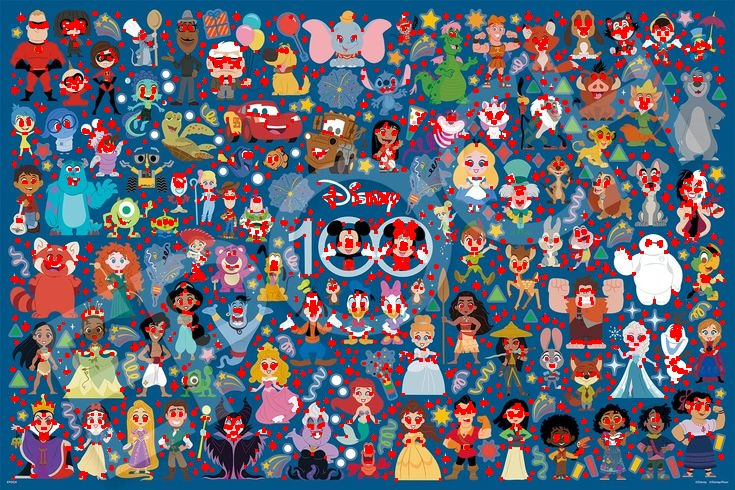
\includegraphics[width=\textwidth]{Graphics/bordes_disney.jpg}
		\captionof*{figure}{Bordes Disney}
	\end{minipage}
	\hfill
	\begin{minipage}[hb]{0.3\textwidth}
		\centering
		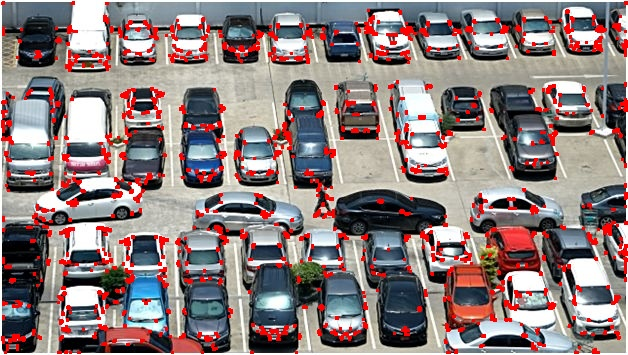
\includegraphics[width=\textwidth]{Graphics/bordes_cars.jpg}
		\captionof*{figure}{Bordes Cars}
	\end{minipage}
	\hfill
	\begin{minipage}[hb]{0.3\textwidth}
		\centering
		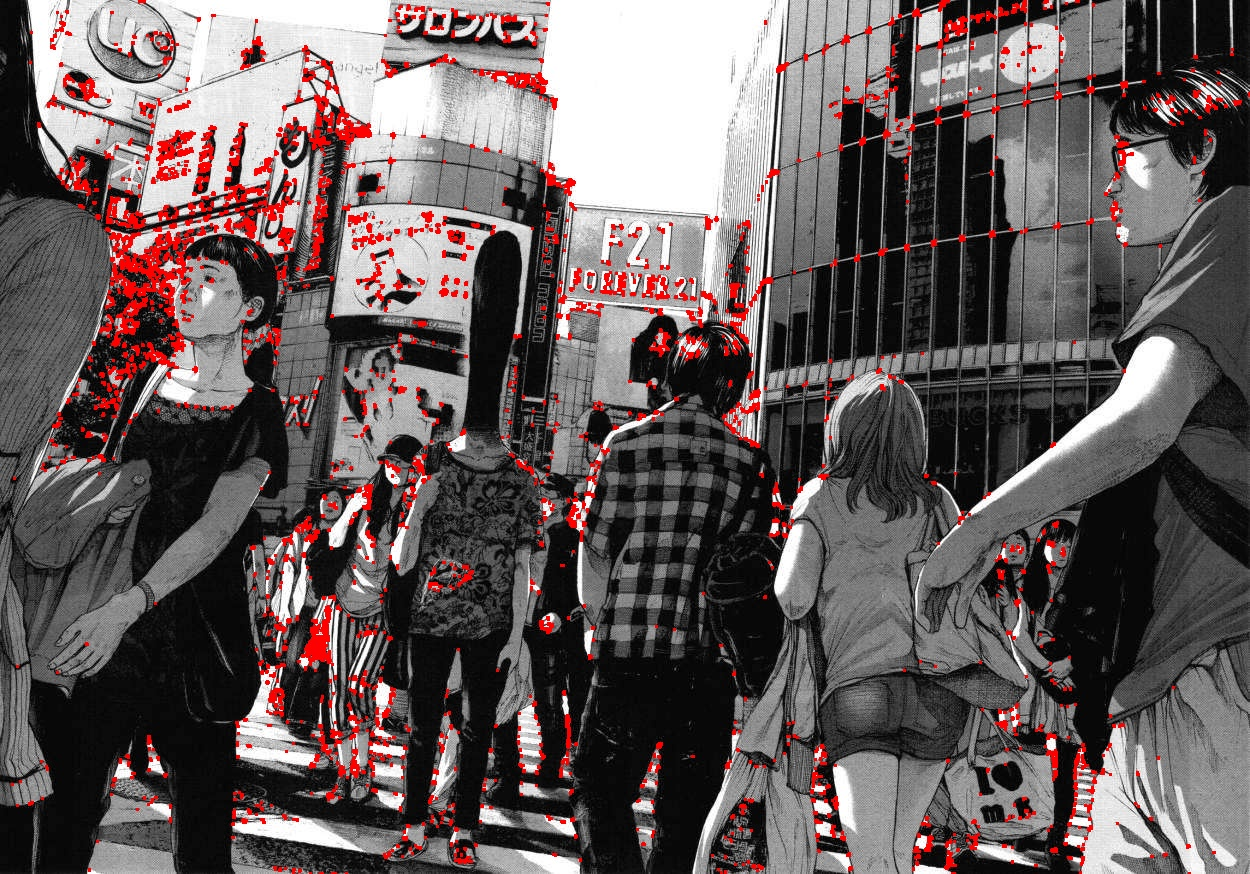
\includegraphics[width=\textwidth]{Graphics/bordes_japan.jpg}
		\captionof*{figure}{Bordes Japan}
	\end{minipage}
	\caption{Imágenes del Sistema con bordes marcados}
	\label{fig:images-borders}
\end{figure}


\subsubsection{Diccionario de ataque basado en segmentaci\'on}
Para la construcción del diccionario de ataque basado en segmentación, se procedió a segmentar las imágenes y determinar sus centros mediante la aplicación del algoritmo \textit{Mean Shift} \cite{Comaniciu2002MeanSA}. A partir de cada segmento obtenido, se utilizó su centro como referencia para generar el diccionario, asegurando que este incorporara la información estructural derivada de la división de cada imagen en sus respectivas regiones. Los resultados de este proceso se muestran en la figura \ref{fig:images-segments }.

\begin{figure}[H]
	\centering
	\begin{minipage}[hb]{0.3\textwidth}
		\centering
		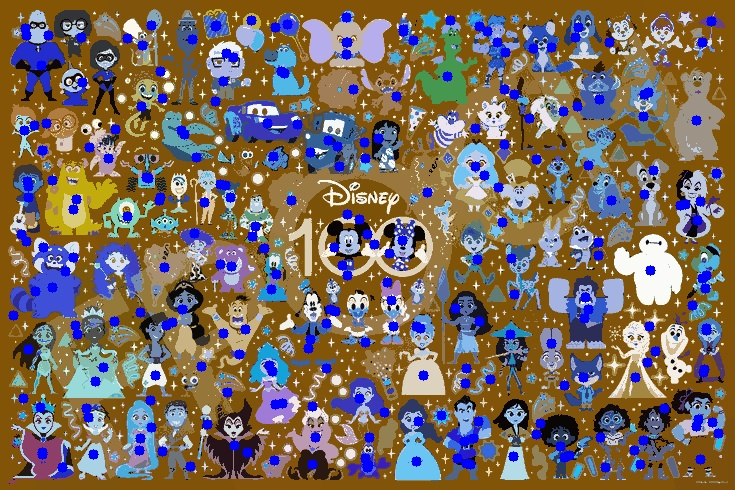
\includegraphics[width=\textwidth]{Graphics/disney-segmented.jpg}
		\captionof*{figure}{Mapa de Segmentaci\'on en imagen Disney}
	\end{minipage}
	\hfill
	\begin{minipage}[hb]{0.3\textwidth}
		\centering
		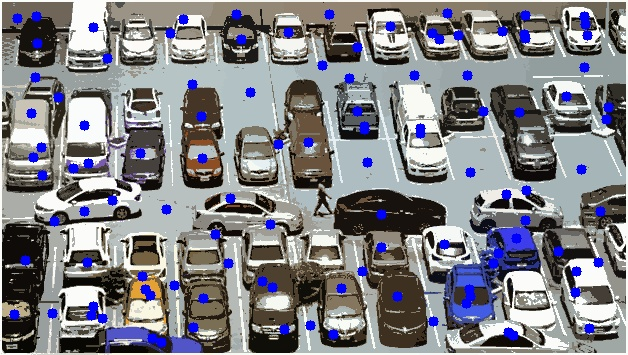
\includegraphics[width=\textwidth]{Graphics/cars-segmented.jpg}
		\captionof*{figure}{Mapa de  segmentaci\'on en imagen Cars}
	\end{minipage}
	\hfill
	\begin{minipage}[hb]{0.3\textwidth}
		\centering
		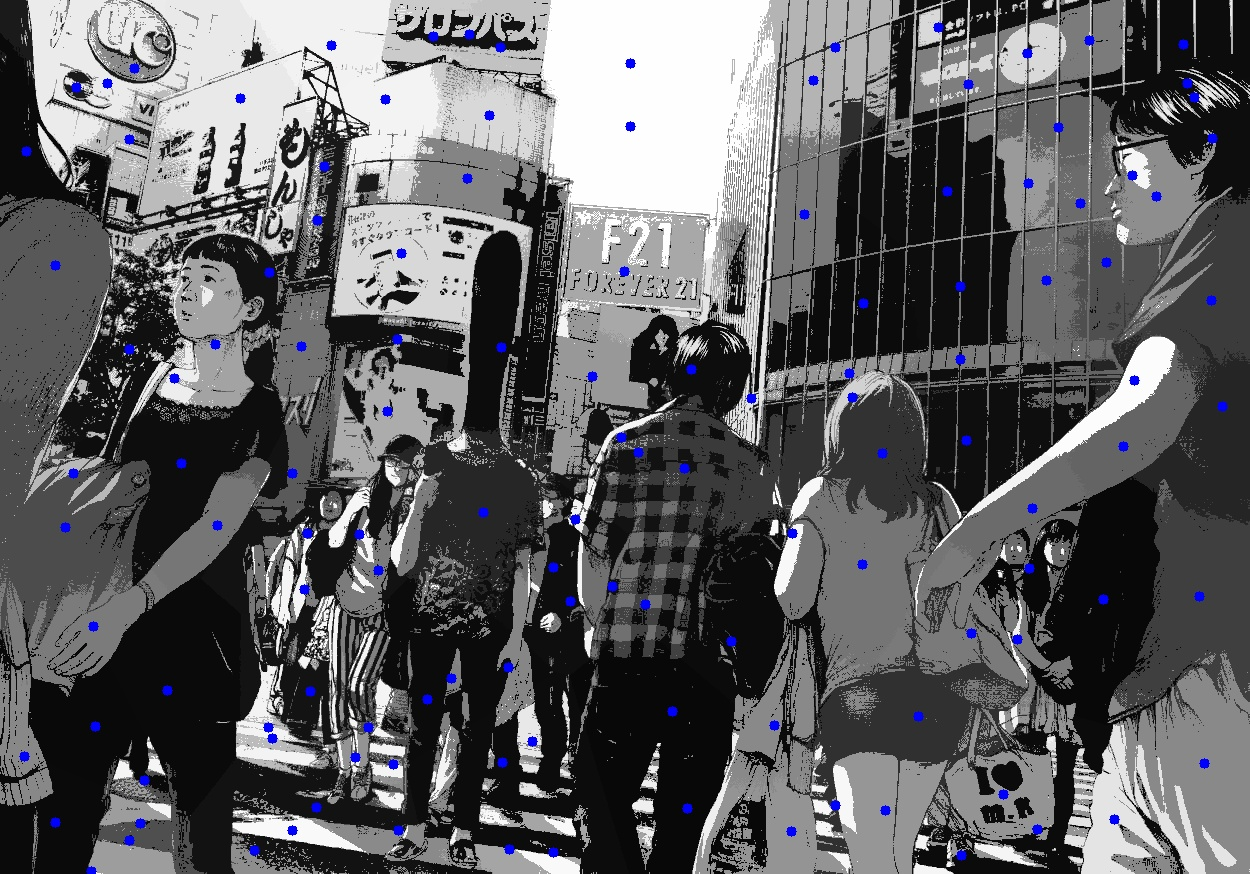
\includegraphics[width=\textwidth]{Graphics/japan-segmented.jpg}
		\captionof*{figure}{Mapa de Segmentaci\'on en imagen Japan}
	\end{minipage}
	\caption{Imágenes del Sistema con sus mapas de segmentaci\'on respectivos y los centros de los mismos marcados}
	\label{fig:images-segments}
\end{figure}

\subsubsection{Diccionario de ataque basado en mapas de atenci\'on visual}
Con el fin de construir el diccionario basado en mapas de atención visual, se calcularon los conjuntos de  puntos m\'as probables a ser seleccionados por los usuarios utilizando un modelo de saliencia visual, el cual modela la forma en que los usuarios miran las im\'agenes. El modelo es el propuesto en \cite{itti2000saliency}, es un modelo \textit{bottom-up}, y se basa en caracter\'isticas como el color, direcci\'on que indica cada pixel y su posici\'on en la imagen. Luego de hallar estos mapas se filtraron sus puntos para determinar los de mayor saliencia visual. Estos fueron utilizados posteriormente en la generaci\'on del diccionario de ataque. Se puede visualizar los puntos seleccionados en las figuras \ref{fig:saliency-map} y \ref{fig:selected-points}.

\begin{figure}[H]
	\centering
	\begin{minipage}[hb]{0.3\textwidth}
		\centering
		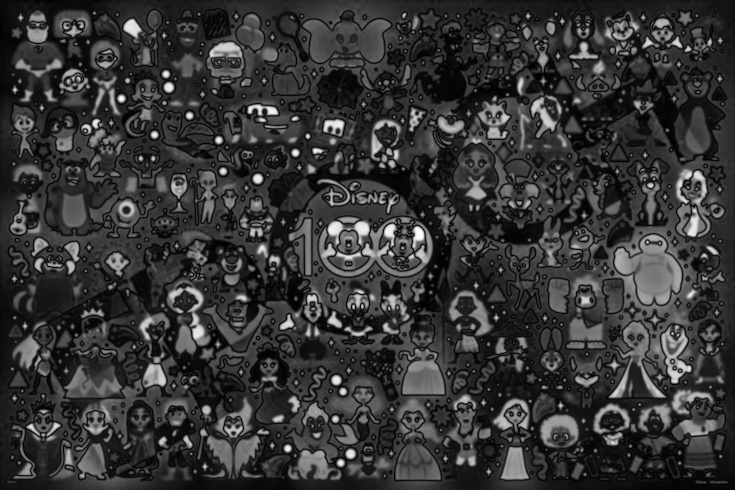
\includegraphics[width=\textwidth]{Graphics/disney-saliency.jpg}
		\captionof*{figure}{Mapa de Atenci\'on en imagen Disney}
	\end{minipage}
	\hfill
	\begin{minipage}[hb]{0.3\textwidth}
		\centering
		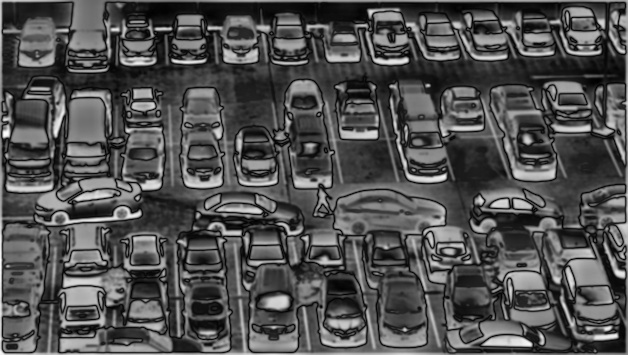
\includegraphics[width=\textwidth]{Graphics/cars-saliency.jpg}
		\captionof*{figure}{Mapa de  Atenci\'on en imagen Cars}
	\end{minipage}
	\hfill
	\begin{minipage}[hb]{0.3\textwidth}
		\centering
		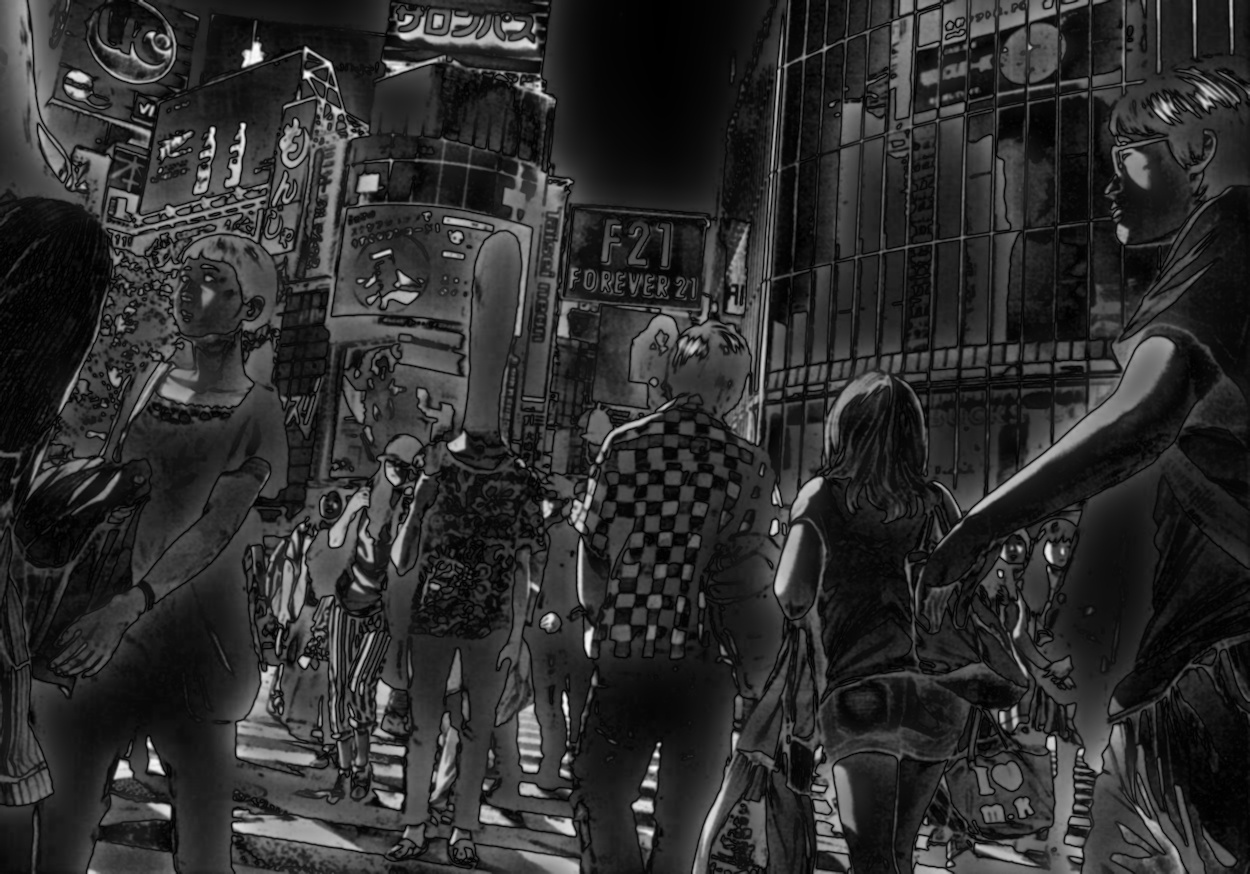
\includegraphics[width=\textwidth]{Graphics/japan-saliency.jpg}
		\captionof*{figure}{Mapa de Atenci\'on en imagen Japan}
	\end{minipage}
	\caption{Imágenes del Sistema con sus mapas de atenci\'on respectivos }
	\label{fig:saliency-map}
\end{figure}

\begin{figure}[H]
	\centering
	\begin{minipage}[hb]{0.3\textwidth}
		\centering
		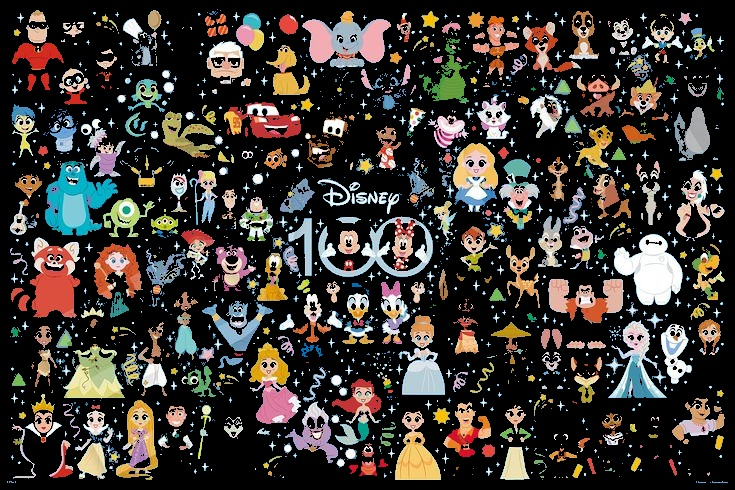
\includegraphics[width=\textwidth]{Graphics/disney-selected-regions.jpg}
		\captionof*{figure}{Regiones seleccionadas en imagen Disney}
	\end{minipage}
	\hfill
	\begin{minipage}[hb]{0.3\textwidth}
		\centering
		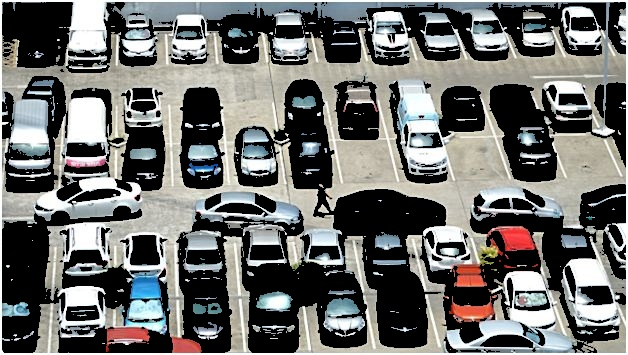
\includegraphics[width=\textwidth]{Graphics/cars-selected-regions.jpg}
		\captionof*{figure}{Regiones seleccionadas en imagen Cars}
	\end{minipage}
	\hfill
	\begin{minipage}[hb]{0.3\textwidth}
		\centering
		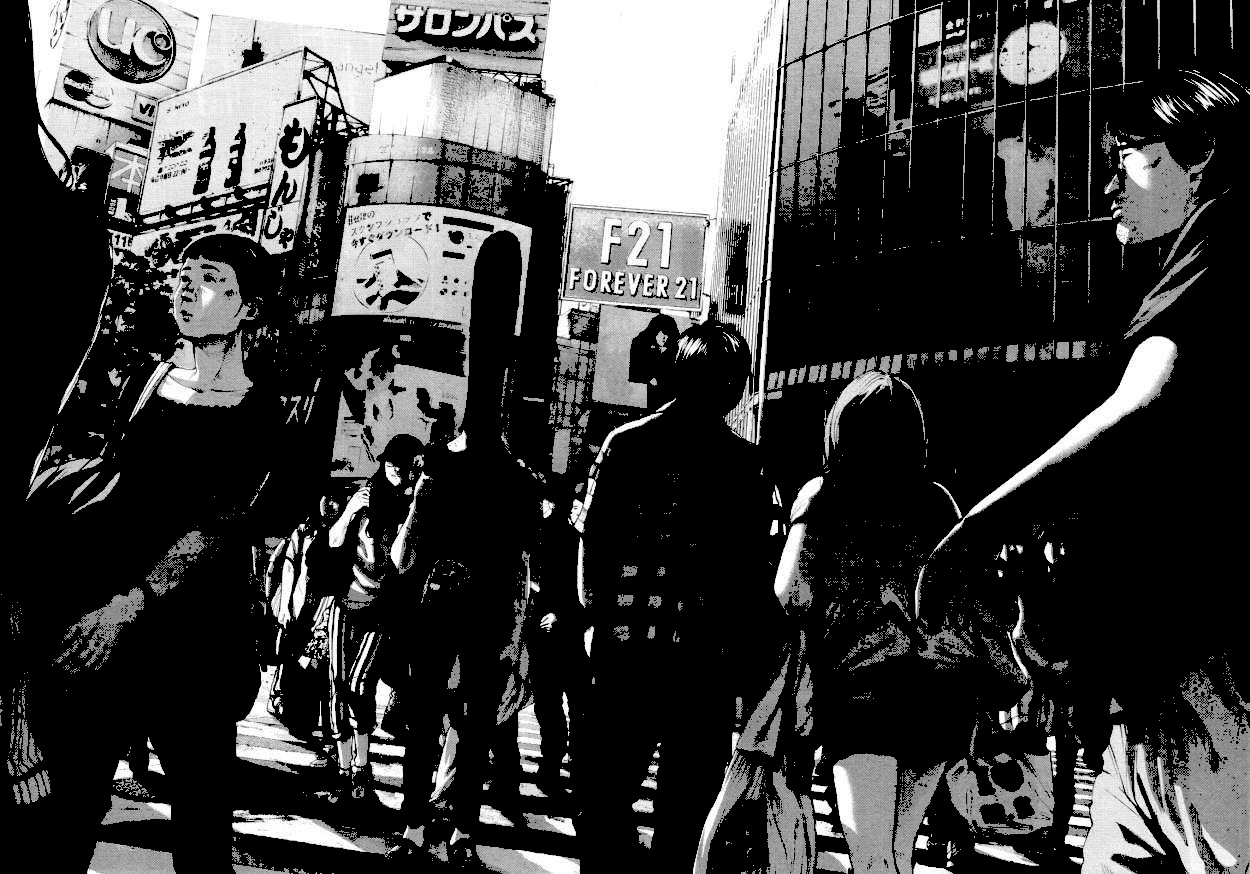
\includegraphics[width=\textwidth]{Graphics/japan-selected-regions.jpg}
		\captionof*{figure}{Regiones seleccionadas en imagen Japan}
	\end{minipage}
	\caption{Imágenes del Sistema con sus respectivas regiones seleccionadas para la creaci\'on del diccionario de ataque}
	\label{fig:selected-points}
\end{figure}


\subsection{Clusterizaci\'on de los puntos }
Para eliminar los puntos que est\'en suficientemente cercanos para caer en la misma regi\'on de tolerancia y reducir las dimensiones de los diccionarios de ataque finales generados, se utiliza el algoritmo de clusterizaci\'on de ventana propuesto en \cite{van2010purely}. Este toma los puntos pertenecientes a una ventana de tama\~no fijo y los sustituye por el pixel del centro geom\'etrico de la ventana. Esto permite eliminar puntos innecesarios y reducir la dimensi\'on del espacio de puntos a analizar para generar un diccionario de ataque final. Para estos fines se tom\'o como tama\~no de ventana $3*r$, donde r es el radio de tolerancia de la imagen en p\'ixeles, dando un margen mayor al generado por la regi\'on original que ser\'ia de $2*r$. Esto permiti\'o reducir la cantidad de puntos a analizar, sin perder mucha informaci\'on. En la tabla \ref{points:void} se puede ver la cantidad de puntos extra\'idos de cada imagen utilizando las t\'ecnicas de procesamiento anteriormente enunciadas. En la tabla \ref{points:cluster} se puede observar la reducci\'on sustancial de la cantidad de puntos despu\'es de aplicar el clusterizado de ventana.
\begin{table}[H]
	\centering
	\caption{Puntos Obtenidos sin clusterizar}
	\label{points:void}
	\begin{tabular}{|l|l|l|l|l|l|l|l|l|l|}
		\hline
		\textbf{im\'agenes/puntos} & \textbf{segmentos } & \textbf{esquinas} & \textbf{saliencia}
		\\ \hline
		\textbf{disney} & 249 & 30 785 & 92 981 \\ \hline
		\textbf{cars} & 110 & 17 826 & 39 764 \\ \hline
		\textbf{japan} & 126 & 47 415 & 203 804  \\ \hline
	
	\end{tabular}
\end{table}

\begin{table}[H]
	\centering
	\caption{Puntos Obtenidos despu\'es de clusterizar}
		\label{points:cluster}
	\begin{tabular}{|l|l|l|l|l|l|l|l|l|l|}
		\hline
		\textbf{im\'agenes/puntos} & \textbf{segmentos} & \textbf{esquinas} & \textbf{saliencia }  \\ \hline
		\textbf{disney} & 36 & 103 & 65  \\ \hline
		\textbf{cars} & 26 & 98 & 38  \\ \hline
		\textbf{japan} & 30 & 82 & 64 \\ \hline
	\end{tabular}
\end{table}

\section{Diccionario de ataque basado en los patrones DIAG y LINE}
Para obtener los diccionarios de ataque que se utiliz\'o el algoritmo basado en grafos propuesto en \cite{van2010purely}. Dicho algoritmo utiliza heur\'isticas para generar contrase\~nas no aleatorias que sigan los patrones DIAG y LINE \cite{s22051987},  comunmente seleccionadas por los usuarios. Para esto se precomputa una matriz de adyacencia M donde para los pares de puntos $i,j \in A$, donde $A$ es un alfabeto de puntos, se cumple.
\[
 M[i,j] = 
\begin{cases} 
	1 & \text{si } (i, j) \in \text{Patrón DIAG o LINE} \\
	0 & \text{si no}
\end{cases}
, \quad \text{para } i,j \in A
\] 

En el caso de la generaci\'on de los grafos utilizados en este ataque se utiliz\'o el par\'ametro de $\tau=9$ que da patrones de relajaci\'on normales, seg\'un \cite{van2010purely} y la distancia m\'axima entre puntos ($Td = \infty$), lo que genera patrones m\'as ce\~nidos a la heur\'istica, en la Tabla \ref{graphs},  se observan los grafos generados para estas im\'agenes con los par\'ametros anteriormente enunciados y el patr\'on DIAG.



\begin{table}[H]
	\centering
	\begin{tabular}{|c|c|c|c|}
		\hline
		& Disney & Cars & Japan \\ \hline
		Segmentos & 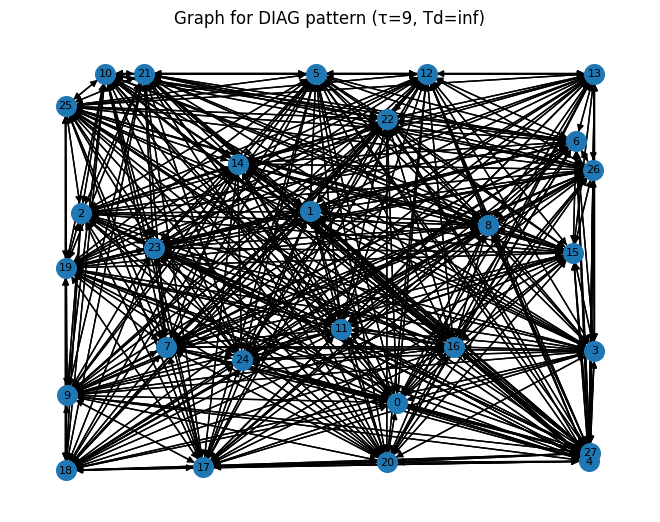
\includegraphics[width=3.5cm]{Graphics/disney-cluster-graph.png} 
		& 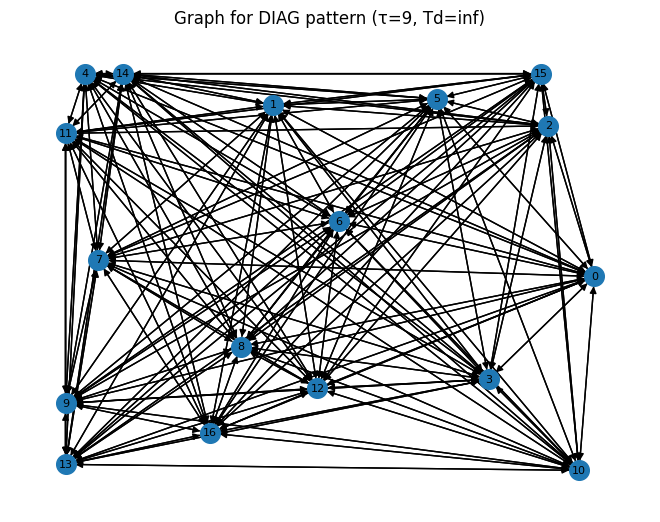
\includegraphics[width=3.5cm]{Graphics/cars-cluster-graph.png} 
		& 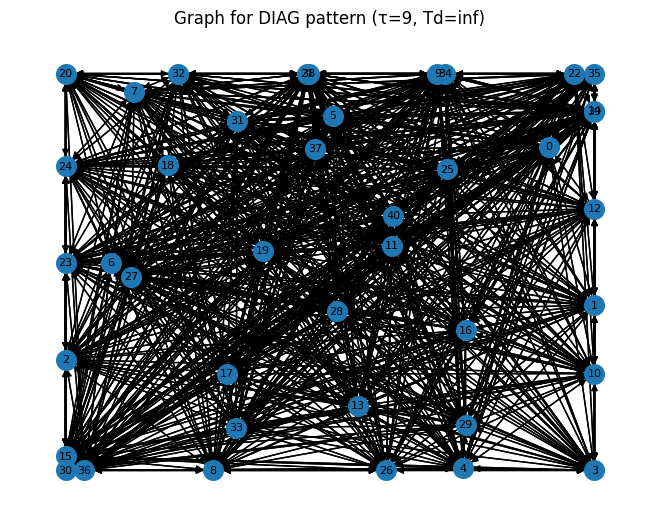
\includegraphics[width=3.5cm]{Graphics/japan-cluster-graph.png} \\ \hline
		Esquinas  & 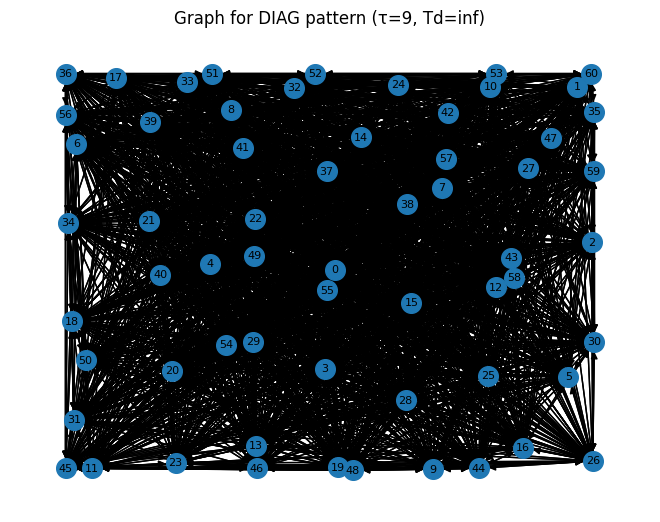
\includegraphics[width=3.5cm]{Graphics/disney-corner-graph.png} 
		& 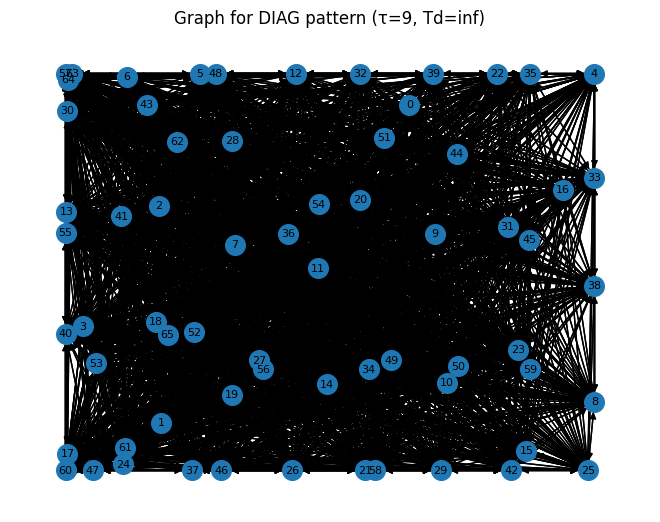
\includegraphics[width=3.5cm]{Graphics/cars-corner-graph.png} 
		& 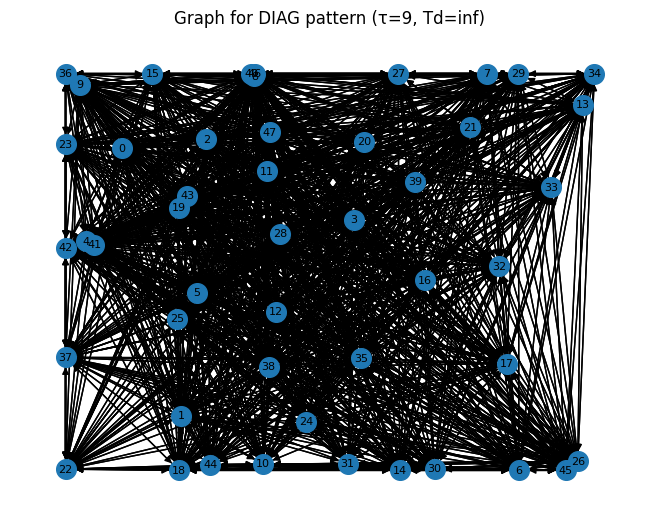
\includegraphics[width=3.5cm]{Graphics/japan-corner-graph.png} \\ \hline
		Saliencia & 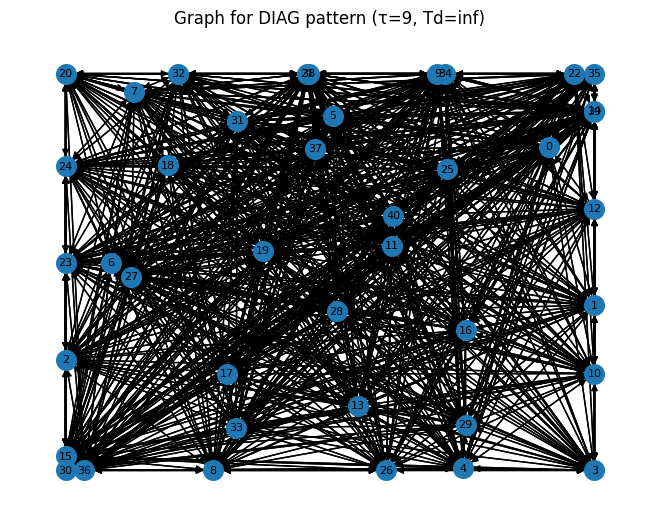
\includegraphics[width=3.5cm]{Graphics/disney-saliency-graph.png} 
		& 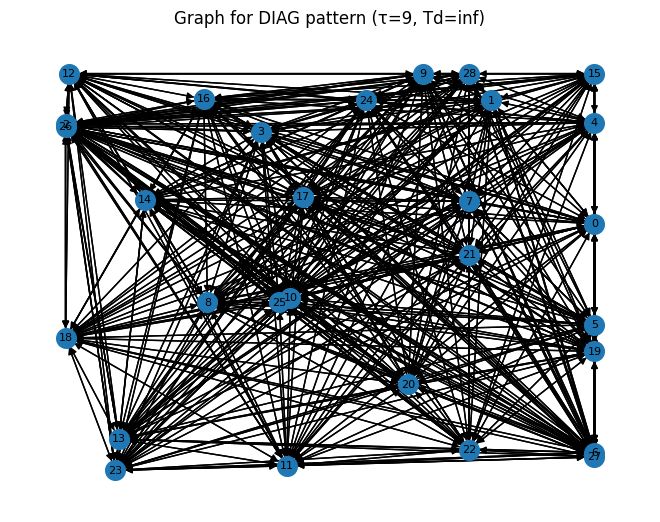
\includegraphics[width=3.5cm]{Graphics/cars-saliency-graph.png} 
		& 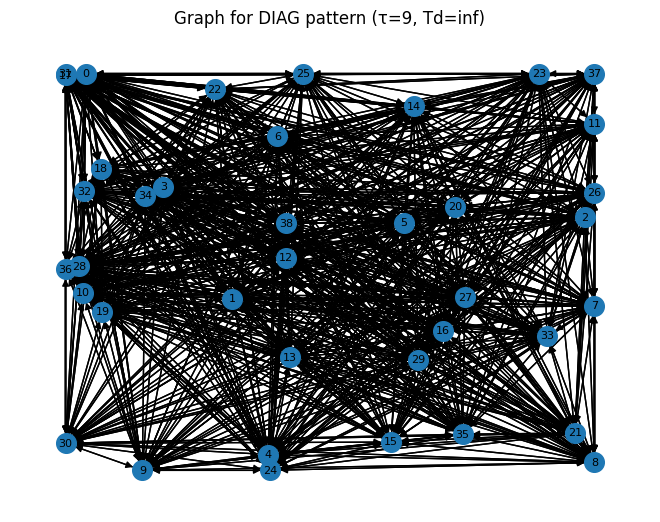
\includegraphics[width=3.5cm]{Graphics/japan-saliency-graph.png} \\ \hline
	\end{tabular}
	\caption{Grafos obtenidos para cada conjunto de puntos y el patr\'on DIAG}
	\label{graphs}
\end{table}


Para una mejor separaci\'on dichas heur\'isticas, se separaron los patrones en sub heur\'isticas, ver en \cite{van2010purely}, que disminuye la complejidad de implementar las comprobaciones de cada par de puntos. Luego para generar los diccionarios de ataque solo se necesita hallar los caminos de tama\~no 5 del grafo (ciclos inclu\'idos), en este caso se utiliz\'o DFS \textit{Depht First Search}, (B\'usqueda en profundidad), iterativo, guardando continuamente los resultados en archivos usando el formato \textit{JSON lines}. Esto permiti\'o reducir el requerimiento memoria ram por parte del sistema y tener una generaci\'on  din\'amica ya que el estado del DFS se guarda en el archivo. El tiempo de generaci\'on de dichos diccionarios oscil\'o de 2 a 3 horas cada uno, llegando a obtener archivos de 21GB de contrase\~nas, en la tabla \ref{dictionary:lengths} se pueden ver la cantidad de contrase\~nas generadas en cada diccionario.  

\begin{table}[H]
	\centering
	\caption{Tama\~no de los diccionarios obtenidos}
	\label{dictionary:lengths}
	\begin{tabular}{|l|l|l|l|l|l|l|l|l|l|}
		\hline
		\textbf{im\'agenes/contrase\~nas} & \textbf{segmentos} & \textbf{esquinas} & \textbf{saliencia }  \\ \hline
		\textbf{disney} & 14 880 348 & 389 469 380 & 104 960 000  \\ \hline
		\textbf{cars} & 1 114 112 & 558 134 287 & 17 825 024  \\ \hline
		\textbf{japan} & 5 387 888 & 3 894 822 & 81 320 304 \\ \hline
	\end{tabular}
\end{table}


\section{Ejecuci\'on del ataque}


Una vez generados los diccionarios, se procedió a la autenticación de cada usuario utilizando las contraseñas contenidas en los diccionarios de ataque. Para agilizar el proceso, esta tarea se realizó de manera asíncrona, como se ilustra en los ejemplos de código \ref{attack1} y \ref{attack}. No obstante, el ataque resultó infructuoso, ya que ninguna contraseña pudo ser vulnerada. Lo que significa que la muestra de las contrase\~nas seleccionadas por los usuarios no deben seguir patrones DIAG y LINE. Sin embargo, esto no quiere decir que est\'en absentas de alg\'un otro patr\'on no aleatorio. Por ende, en trabajos futuros se le a\~nadir\'a a la iplementaci\'on propuesta, los \textit{tests} existentes en la bibliograf\'ia para la detecci\'on de contrase\~nas que carezcan de aleatoriedad.
\bigskip\bigskip
\begin{lstlisting}[style=mystyle, language=Python, caption=C\'odigo del ataque, label=attack1][H]
data = (
supabase
.table('passwords')
.select('image, tolerance, user_id(email)')
.not_.is_('user_id', 'null')
.execute()
).data

results = {}

if not data:
 print("No se encontraron registros")
 exit()
threads=[]
for password in data:
  thread = Thread(target=predict_password,args=(password,))
  thread.start()
  threads.append(thread)
for thread in threads:
  thread.join()
\end{lstlisting}

\clearpage

\begin{lstlisting}[style=mystyle, language=Python, caption=C\'odigo que se ejecuta en cada hilo del ataque, label=attack][hb]
def predict_password(password):
 base_path = os.path.join("[ruta a las im\'agenes]", password['image'])  # Directorio base organizado
 email = password['user_id']['email'] if isinstance(password['user_id'], dict) else None

 #Aqui se guardar\'an los intentos de autenticaci\'on realizados
 with lock:
  results[email] = {
	'cluster_tries': 0,
	'corner_tries': 0,
	'saliency_tries': 0
  }

 file_types = {
	'saliency': 'saliency_dictionary.json',
	'cluster': 'cluster_dictionary.json',
	'corner': 'corner_dictionary.json'	
 }

 for key, filename in file_types.items():
  file_path = os.path.join(base_path, filename)
  with jsonlines.open(file_path) as points_data:
   for points in points_data:
     results[email][f'{key}_tries'] += 1

  passpoints = {
	'points': list(map(lambda x: {'x':x[0],'y':x[1]},points)),
	'tolerance': password['tolerance'],
	'image': {
		'name': password['image']
	}
  }

  # 8. Llamada a \textit{Supabase}  
  response = supabase.functions.invoke(
  "passpoints-login",
     invoke_options={
    	"body": {
		'email': email,
		'password': passpoints
 	  }
   }
  )
  resp = json.loads(response)
  if resp['success']:
   return {'success':True,'results':results[email]}
\end{lstlisting}
